\documentclass[12pt,a4paper]{article}
\usepackage[hidelinks]{hyperref}
\usepackage[cm]{fullpage}
\usepackage{graphicx}
\usepackage{feynmp}
\usepackage{amsmath}
\usepackage{amssymb}
\DeclareGraphicsRule{*}{mps}{*}{}
\usepackage{caption}
\usepackage{subcaption}
\usepackage{slashed}
\usepackage[utf8]{inputenc}

%\usepackage{lineno}
%\linenumbers

\begin{document}
\begin{fmffile}{feynmandiags}

\title{Systematic uncertainty studies in the search for Higgs boson decays to invisible final states and the combination of Higgs boson decay channels at the Compact Muon Solenoid}
\author{Patrick Dunne \\ Imperial College London \\ Supervisors: David Colling, Gavin Davies}
\maketitle


\renewcommand{\abstractname}{\vspace{-\baselineskip}}
\begin{abstract}
  An overview of Higgs boson analyses at the Compact Muon Solenoid (CMS) is presented, with the two projects the author is involved in described in more detail. The first project is the measurement of a 95\% confidence level on the branching fraction of the Higgs boson to invisible final states, with a particular emphasis on the estimation of the systematic uncertainties due to the jet energy scale and resolution in the W + jets background. The second project is a method for increasing the reliability of and reducing the time taken to perform profiled maximum likelihood fits in the combination of CMS results from several Higgs boson decay modes by `pruning' of systematic uncertainties.
\end{abstract}

\newpage

\tableofcontents

\newpage

\section{Introduction}
\subsection{Theoretical background}
\label{theory}
\subsubsection{The Standard Model}
\label{SM}

The Standard Model (SM) of particle physics is one of the most successful physical theories devised, and one of its cornerstones is electroweak unification \cite{glashow,weinberg,salam}. Electroweak unification proposes that the Lagrangian has an SU(2)xU(1) symmetry and local gauge invariance with four gauge bosons, the photon ($\gamma$) and the $W^{\pm}$ and $Z$ bosons. The $W$ and $Z$ bosons, were observed at the UA1 and UA2 experiments in 1983 \cite{wdiscovery,zdiscovery}, with masses of 80.4 GeV and 91.2 GeV, respectively. It was already known that massive exchange particles would be required to explain the short range of the weak force. Unfortunately the symmetry of the Lagrangian is broken by introducing mass terms for the vector bosons, so a different mechanism is required to give mass to the particles we observe.

The Higgs mechanism provides a solution to this problem by adding a complex scalar field with a non-zero vacuum expectation value, the Higgs field, to the Lagrangian that couples to the gauge bosons \cite{englertbrout,higgs1,higgs2,guralniketc,higgs3,kibble}. While the Lagrangian term itself respects the symmetry described above, the ground state does not; this is called spontaneous symmetry breaking. The gauge bosons coupling to a field with a vacuum expectation value accounts for their mass, and we are left with the prediction of a new massive scalar boson, the Higgs boson. A candidate Higgs boson has recently been discovered by the ATLAS and CMS \cite{atlasdiscovery,cmsdiscovery} experiments at CERN the CERN LHC \cite{lhc}.

The Higgs mechanism can also explain the fermion masses by introducing a Yukawa coupling between the Higgs field and the fermions, the mass would be expected to be proportional to the strength of the coupling. Measuring the strength of the coupling of the 125 GeV Higgs-candidate boson that has been discovered at the LHC to fermions will therefore be important in confirming whether it is a SM Higgs boson. It is important to note that the theory does not predict the particles' masses.

\begin{figure}[h]
  \centering
  \raisebox{-0.5\height}{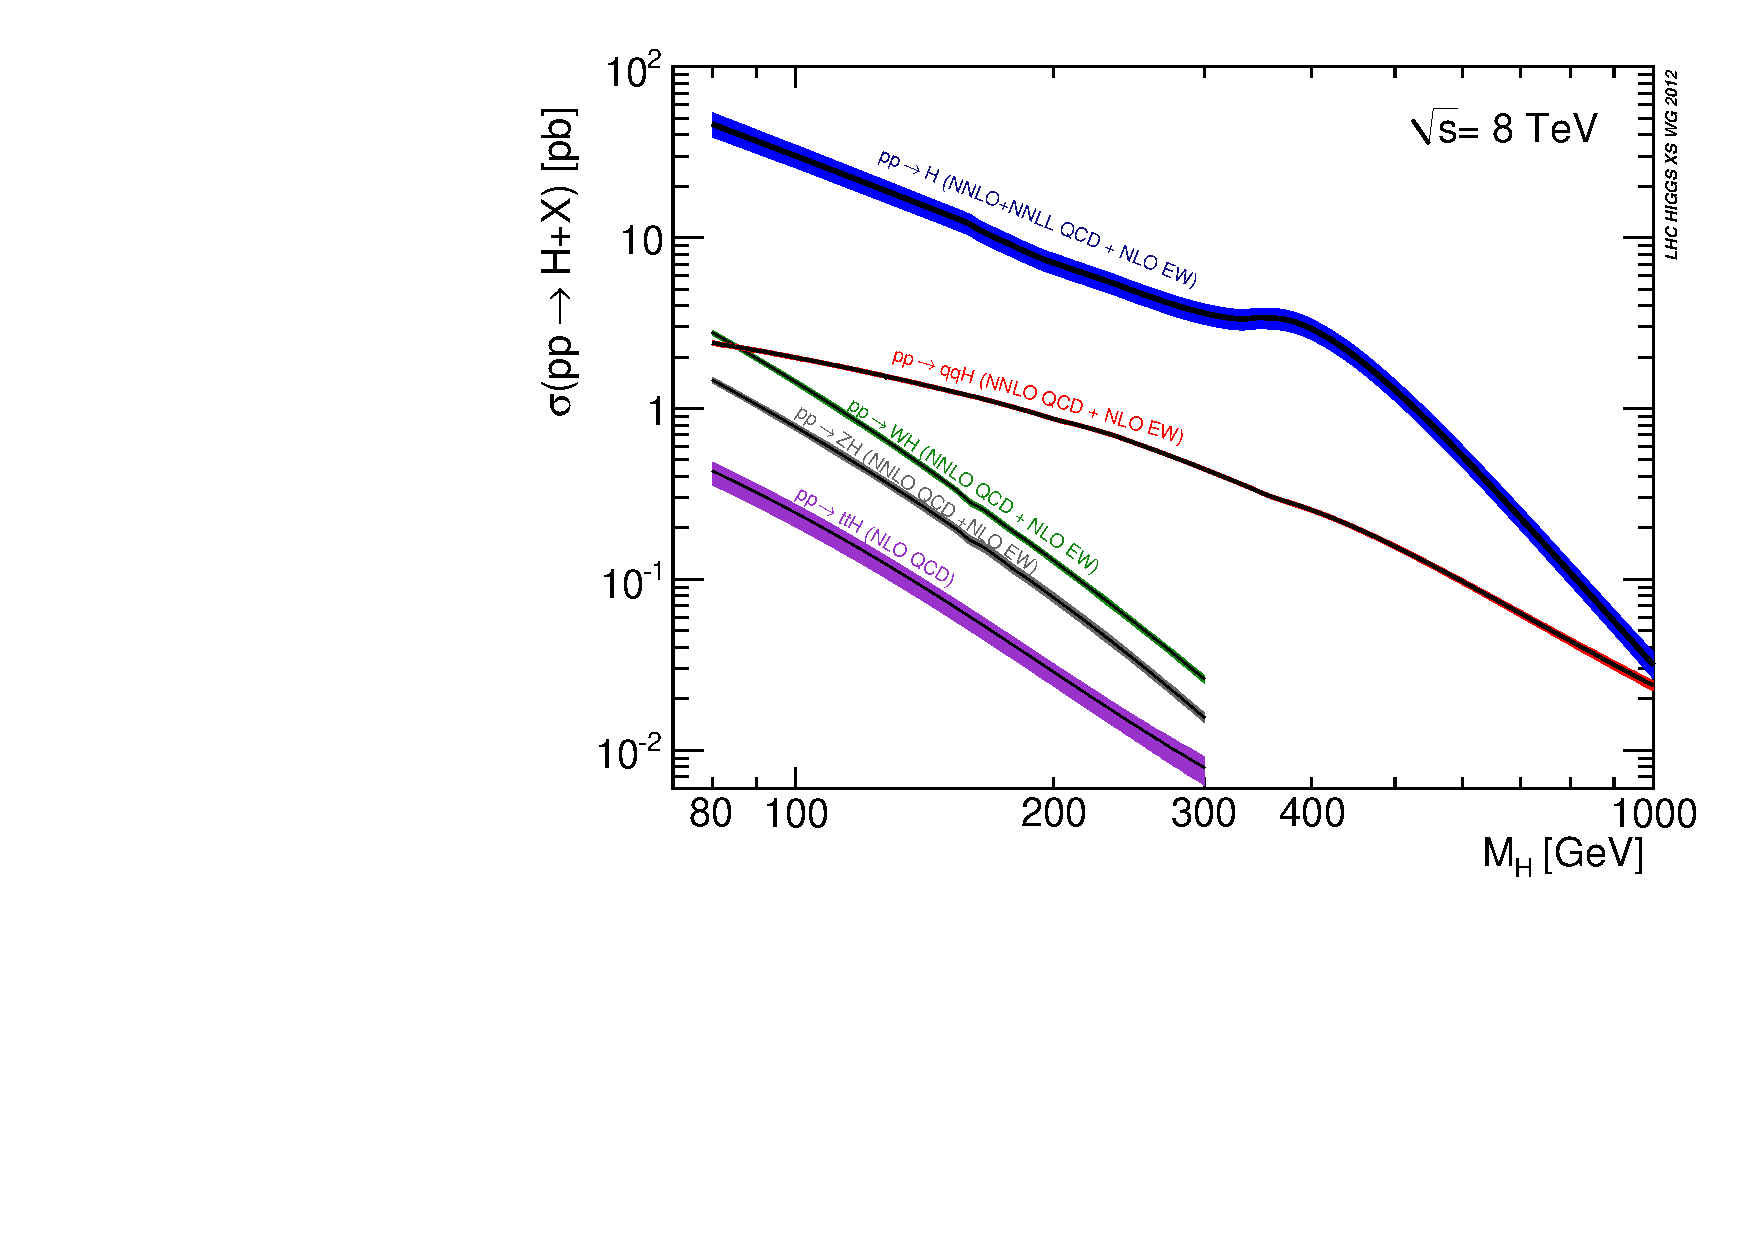
\includegraphics[width=0.49\textwidth,height=0.35\textheight]{Images/Higgs_XS_8TeV_lx.pdf}}
  \raisebox{-0.5\height}{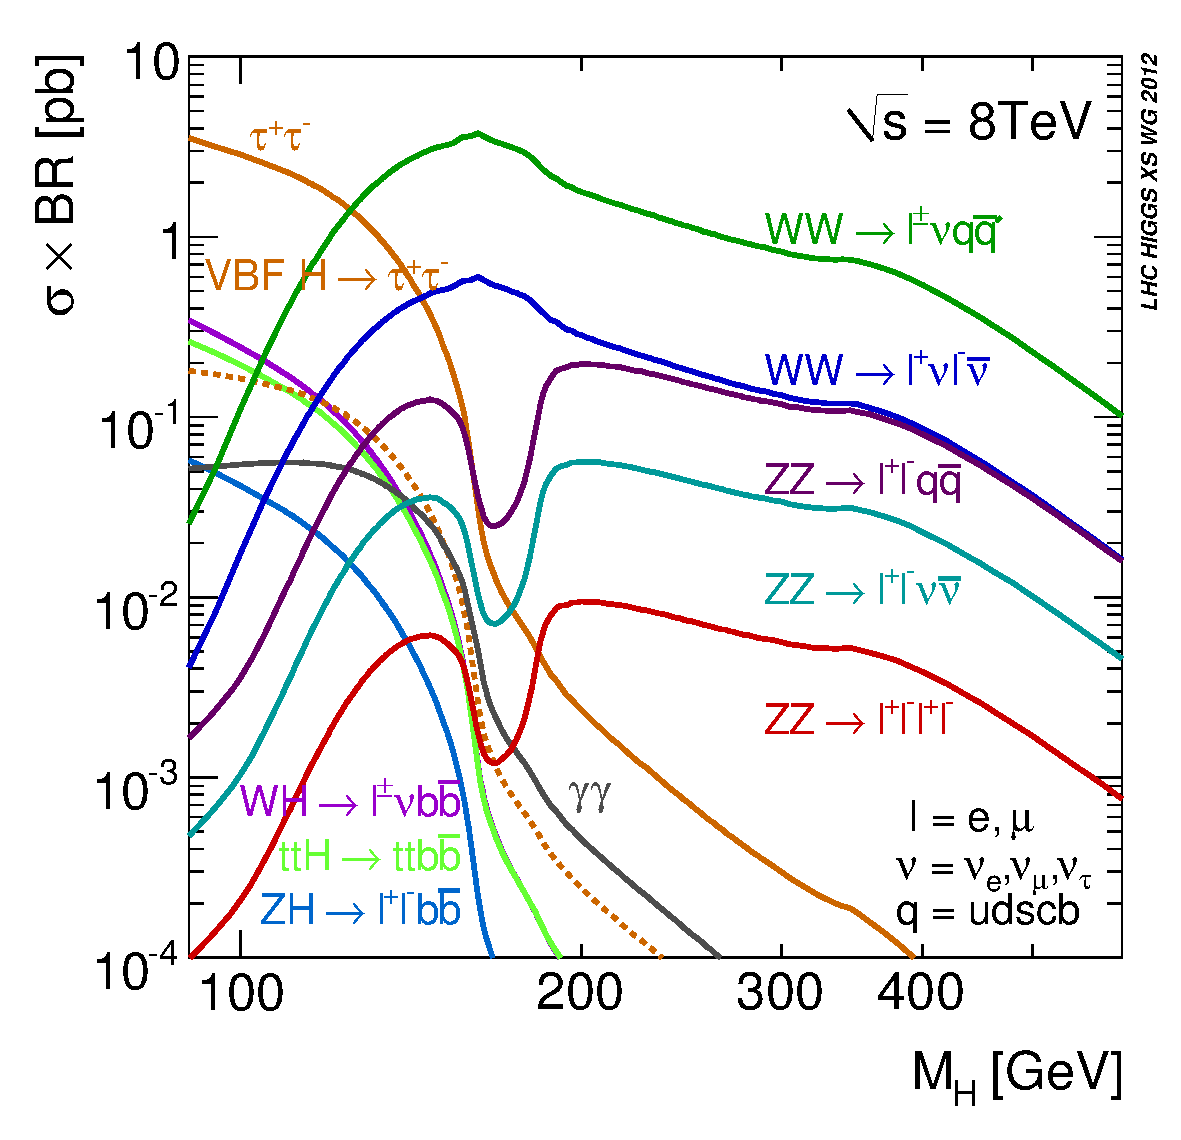
\includegraphics[width=0.49\textwidth,height=0.35\textheight]{Images/XSBR_8TeV_SM.pdf}}
  \caption{Left: cross-section for SM Higgs boson production mechanisms, $pp \rightarrow H$ is gluon fusion, $pp \rightarrow qqH$ is VBF and the remaining three are associated production with $W$ and $Z$ bosons and $t\bar{t}$. Right: the branching fractions multiplied by the production cross-section for the decay modes of the SM Higgs boson. (From \cite{lhchxswg})}
  \label{higgbrfig}
\end{figure}


\begin{figure}
  \centering
  \begin{subfigure}{0.24\textwidth}
    \centering
    %ggf 
    \begin{fmfgraph*}(75,100)
      \fmfleft{i0,i1,i2,i3,i4,i5}
      \fmfright{o1}
      \fmf{gluon}{i1,v1}
      \fmf{gluon}{i4,v2}
      \fmf{fermion,tension=0}{v1,v2}
      \fmf{fermion,tension=2/3}{v2,v3,v1}
      \fmf{dashes}{v3,o1}
      \fmflabel{$g$}{i1}
      \fmflabel{$g$}{i4}
      \fmflabel{$H$}{o1}
    \end{fmfgraph*}
    \caption{}
  \end{subfigure}
  \begin{subfigure}{0.24\textwidth}
    \centering
    %vbf                                                                                                   
    \begin{fmfgraph*}(75,100)
      \fmfleft{i1,i2}
      \fmfright{o1,o2,o3}
      \fmf{fermion}{i1,v1,o1}
      \fmf{fermion}{i2,v2,o3}
      \fmf{photon,label=$W,,Z$}{v1,v3}
      \fmf{photon,label=$W,,Z$}{v2,v3}
      \fmf{dashes}{v3,o2}
      \fmflabel{$q$}{i1}
      \fmflabel{$q$}{i2}
      \fmflabel{$q$}{o1}
      \fmflabel{$q$}{o3}
      \fmflabel{$H$}{o2}
    \end{fmfgraph*}
    \caption{}
  \end{subfigure}
  \begin{subfigure}{0.24\textwidth}
    \centering
    %Higgstrahlung
    \begin{fmfgraph*}(75,100)
      \fmfleft{i1,i2}
      \fmfright{o1,o2}
      \fmf{fermion}{i1,v1}
      \fmf{fermion}{v1,i2}
      \fmf{photon,label=$W,,Z$}{v1,v2}
      \fmf{photon}{v2,o1}
      \fmf{dashes}{v2,o2}
      \fmflabel{$q$}{i1}
      \fmflabel{$\bar{q}$}{i2}
      \fmflabel{$W,Z$}{o1}
      \fmflabel{$H$}{o2}
    \end{fmfgraph*}
    \caption{}
  \end{subfigure}
  \begin{subfigure}{0.24\textwidth}
    \centering
    %ttH                                                                                                    
    \begin{fmfgraph*}(75,100)
      \fmfleft{i0,i1,i4,i5,i6,i2,i3}
      \fmfright{o0,o1,o2,o3,o4}
      \fmf{gluon,tension=3/2}{i1,v1}
      \fmf{gluon,tension=3/2}{i2,v2}
      \fmf{fermion}{o1,v1,v3,v2,o3}
      \fmf{dashes,tension=3/2}{v3,o2}
      \fmflabel{$g$}{i1}
      \fmflabel{$g$}{i2}
      \fmflabel{$\bar{t}$}{o1}
      \fmflabel{$t$}{o3}
      \fmflabel{$H$}{o2}
    \end{fmfgraph*}
    \caption{}
  \end{subfigure}
  \caption{The Feynman diagrams for the Higgs production mechanisms at CMS are shown: a) gluon fusion, b) vector boson fusion, c) $W$/$Z$ associated production and d) $t\bar{t}$ associated production.}
  \label{higgprodfig}
\end{figure}

\subsubsection{SM Higgs production and decay mechanisms}
\label{proddec}

Fig.~\ref{higgbrfig} shows the SM Higgs boson's main production methods and their cross-sections. It can be seen that the production mechanism with the highest cross-section at the LHC is gluon fusion which proceeds through a quark loop as shown in Fig.~\ref{higgprodfig}a. Because the Higgs couples to mass this loop is dominated by the top quark contribution, although all strongly interacting massive particles contribute.

After gluon fusion the next highest production cross-section is for vector boson fusion (VBF), which occurs through the Feynman diagram shown in Fig.~\ref{higgprodfig}b. VBF has the advantage that the two quarks in the final state are produced with a large pseudorapidity (defined in Sec.~\ref{cmslhc}) gap between them. This gap can be used as an experimental signature for these events \cite{zeppenfeld}.

Finally there is associated production, where the Higgs is produced along with other particles, predominantly $W$ or $Z$ bosons and $t\bar{t}$ pairs through the diagrams in figs.~\ref{higgprodfig}c and \ref{higgprodfig}d. These channels are useful because the leptons produced when the particles produced with the Higgs decay can be used to trigger, which significantly reduces backgrounds and thus increases the purity of the selected samples. Furthermore the rate for these processes is lower allowing the trigger to be designed with a higher efficiency.

As the Higgs boson couples proportionally to mass, it would be expected that the dominant decays would be to heavy particles. At a mass around 125 GeV the heaviest particle that can be pair produced on-shell is the b quark. However, large QCD multijet backgrounds make it impossible to perform a Higgs search in the $b\bar{b}$ channel, because there is nothing to trigger on, unless the Higgs was created in associated production, and the background is significantly reduced.

As the mass increases decays to two $W$ or $Z$ bosons become increasingly important. It can be seen from Fig.~\ref{higgbrfig} that both the $WW$ and $ZZ$ channels have high branching ratios even at 125 GeV. This is because, even though two real bosons cannot be created, it is possible to produce one real and one virtual boson. When at least one of the bosons decays leptonically the lepton can be used to trigger allowing this search to be carried out for all of the production mechanisms. The $ZZ$ channel is also particularly important because it has several fully leptonic final states which allow full kinematic reconstruction giving it a very good mass resolution \cite{cmsdiscovery}.

The other channel with very good mass resolution is the decay to two photons ($\gamma\gamma$), which also has a final state that can be fully reconstructed and is easy to trigger on. The $\gamma\gamma$ decay proceeds through a similar loop diagram to gluon fusion, but with the gluons replaced with photons and any massive charged particle in the loop. The $\gamma\gamma$ decay also has most sensitivity at low mass because at higher masses decays to $WW$, $ZZ$ and, at very high Higgs mass, $t\bar{t}$ are dominant. 

The final channel that is being examined for the main Higgs analysis at CMS is the decay to two $\tau$ leptons. Fig.~\ref{higgbrfig} shows that this has a high branching ratio, however when the $\tau$ leptons decay neutrinos are produced with variable energies which means that this channel does not have a good mass resolution. A signal in the $\tau$ channel therefore manifests itself as a broad excess which is difficult to search for. Like the $\gamma\gamma$ channel the decay to $\tau$ leptons is also a channel with most sensitivity in the low mass region.

\subsubsection{Higgs decays to invisible particles}
\label{invtheory}
Despite the great successes of the standard model, it still has several limitations, including the lack of a theory of quantum gravity and the so called `hierarchy problem' \cite{susy}. This means that, whilst the standard model Higgs boson can only decay to invisible final states by decaying to two $Z$ bosons, which subsequently both decay into neutrinos, a process with a vanishingly small cross section compared to backgrounds, searches for Higgs decays to invisible final states (``Higgs to invisible'') are still well motivated theoretically, because several beyond the SM theories predict Higgs decays to long-lived neutral particles \cite{higgworkgroup2001}. 

One example is supersymmetry, which predicts that each SM particle has a heavier `superparticle' partner. In some supersymmetric models the lightest superparticle is stable, neutral and weakly interacting, making it invisible to the CMS detector, yet still interacts with the Higgs boson \cite{susy}. Another example is theories with large extra dimensions, which can also lead to large invisible Higgs boson branching fractions \cite{extradim}. Decays to invisible final states are studied in more detail in Sec.~\ref{htoinv}.

\subsection{CMS and the LHC}
\label{cmslhc}
The LHC is a proton proton collider situated at CERN near Geneva, Switzerland, with a design centre of mass energy ($\sqrt{s}$) of 14 TeV \cite{lhc}. It ran in 2010 and 2011 at $\sqrt{s}$ = 7 TeV, and in 2012 at $\sqrt{s}$ = 8 TeV. The CMS detector is one of the two general purpose detectors at the LHC, the other being ATLAS \cite{atlastdr}. The structure of the CMS detector is shown in Fig.~\ref{detpic}, from the collision point outwards it is made up of: a central silicon detector for vertex location and tracking, an electromagnetic calorimeter, a hadronic calorimeter, a superconducting magnet to bend particle tracks for momentum measurement and a muon system situated in the magnet return yoke \cite{cmstdr}. To date an integrated luminosity of 5.6 fb$^{-1}$ has been recorded by CMS at $\sqrt{s}$ = 7 TeV, and 21.8 fb$^{-1}$ have been collected at $\sqrt{s}$ = 8 TeV

\begin{figure}[hb]
  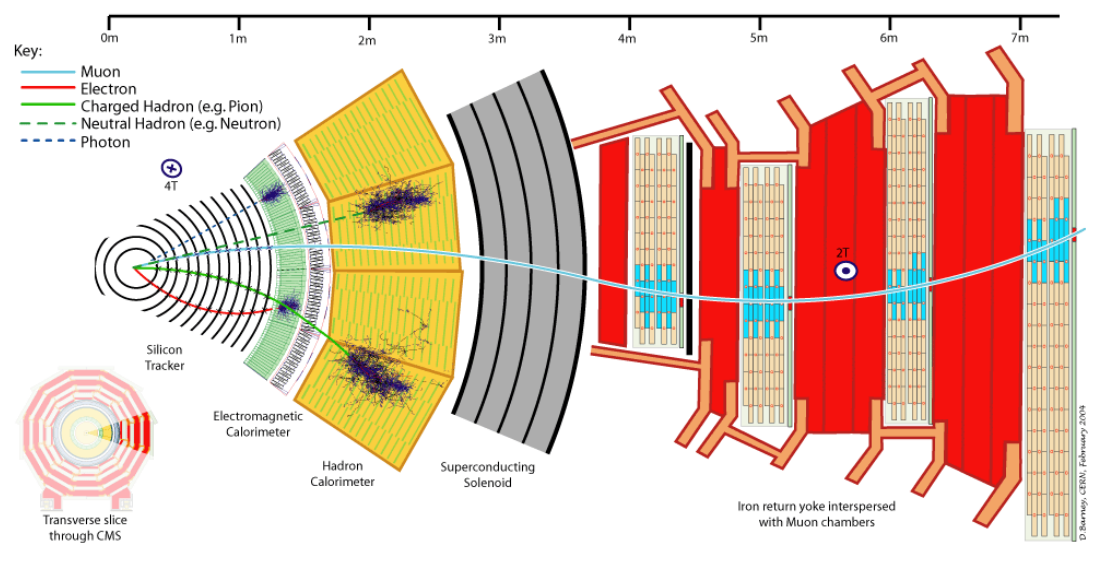
\includegraphics[width=\textwidth]{Images/detpic.png}
  \caption{A schematic slice of the CMS detector showing the main subdetectors}
  \label{detpic}
\end{figure}

\newpage

The co-ordinate system used by CMS is right-handed with the x-axis pointing to the centre of the LHC ring, the y-axis pointing vertically upwards and the z axis along the beam-line. The spherical polar co-ordinates $\theta$ and $\phi$ take their normal definitions. CMS also uses the pseudorapidity variable, $\eta$, which is defined as
\begin{equation}\label{pseudorap}
  \eta = -\ln\tan\left(\frac{\theta}{2}\right).
\end{equation}

All the subdetectors cover the full $2\pi$ range in $\phi$, except for small regions blocked by services such as power cabling and cooling. The pseudorapidity coverage of the subdetectors vary and will be described below.


\subsubsection{The Tracker}
\label{tracker}
The tracker consists of an inner pixel detector and an outer silicon strip detector. Both the pixel and strip detectors are split into a barrel section and endcaps and cover the pseudorapidity range $|\eta| < 2.5$. The pixel detector has a resolution  of ~15 $\mu$m in r-$\phi$ and z giving vertex resolutions of 30-40 $\mu$m in the longitudinal direction, while the strip detector has a resolution in the range 23-52 $\mu$m in r-$\phi$ and 230-530 $\mu$m in z \cite{cmstdr}. This high accuracy allows discrimination between tracks from pileup (particles from interactions other than the interaction of interest) and those from the collision of interest; it also improves the energy resolution of objects reconstructed by matching calorimeter deposits to tracks and allows jets containing b quarks to be tagged by identifying both the primary interaction vertex and the secondary decay vertex of the b particle. The tracker determines particle momentum from the curvature of tracks, achieving a resolution of 1-2\% for 100 GeV particles with $\eta<1.6$ \cite{cmstdr}.

\subsubsection{The Electromagnetic Calorimeter (ECAL)}
\label{ecal}
The ECAL measures the energy of electrons and photons and consists of a homogeneous PbWO$_{4}$ scintillating calorimeter which is split into a barrel section and two endcaps and covers the pseudorapidity range $|\eta|<3.0$. There is also a preshower sampling calorimeter in the endcap regions consisting of layers of lead and silicon strip detectors, this is designed to improve the identification of neutral pions by improving the spatial resolution of the photons coming from their decays. The ECAL resolution is energy dependent and when measured in a test beam is well described by:
\begin{equation}\label{sigmaE}
  \frac{\sigma}{E} = \frac{\alpha}{\sqrt{E}}\sqrt{\rm{GeV}} \oplus \frac{\beta}{E} \oplus \delta\,.
\end{equation}
with $\alpha$ = 2.8\%, $\beta$ = 120 MeV and $\delta$ = 0.3\%, where $\alpha$ is known as the sampling term, as it is due to the statistical error on the number of scintillation photons detected, $\beta$ is a constant term and $\delta$ is a noise term proportional to the energy deposited \cite{cmstdr}.

 The ECAL energy resolution is important in determining the accuracy of any missing energy calculation because a large proportion of jet energy takes the form of photons and charged hadrons, which deposit energy in the ECAL \cite{particleflow}, making it key to Higgs to invisible searches. The sensitivity of the Higgs to $\gamma\gamma$ channel is also very dependent on good ECAL energy resolution.

\subsubsection{The Hadronic Calorimeter (HCAL)}
\label{hcal}
The HCAL is made up of a barrel region and endcaps, covering $|\eta| < 3.0$, and a forward region, covering $3.0<|\eta|<5.0$. The barrel and endcaps are sampling calorimeters composed of interleaved brass and plastic scintillator. The forward HCAL (HF) is a steel and Cherenkov emitting quartz fibre sampling calorimeter. The energy resolution of the HCAL and ECAL combined, which is the figure most important for missing energy determination, is well described by eqn.~\ref{sigmaE} with $\alpha$=121\%, $\beta$=9.5\% and $\delta$=0 \cite{hcal}. The forward HCAL is particularly important for the Higgs to invisible search, and any other VBF analyses, because the large pseudorapidity gap expected means that 80\% of VBF events with a pseudorapidity gap of at least 4.4 will have at least one jet in the forward HCAL \cite{higgworkgroup2001}.

\subsubsection{The muon system}
\label{muon}
The muon system is situated in the return yoke of the superconducting magnet and consists of a drift tube system in the barrel section of the detector and a cathode strip chamber system in the endcap, which have good postion resolution, combined with a resistive plate chamber system both in the endcaps and the barrel, which provides high precision timing information. Together these systems cover the pseudorapidity range $|\eta|<2.4$. Combined with inner tracker information the muon system gives a momentum resolution of $\delta p_{T}$/$p_{T}$ between 0.01 and 0.1 for muons with $p_{T}$ between 10 and 1000 GeV \cite{cmstdr}.

\subsubsection{Triggering and offline computing}
\label{trigcomp}
The rate of the collisions at the LHC is far too great for CMS to record every detected event. During the 2012 run the rate of collisions at the LHC was 20 MHz, so a triggering process is therefore necessary to select the most interesting events. At CMS the trigger consists of the level one (`L1') trigger, which is hardware based, and the higher level trigger (`HLT'), which is software based \cite{cmstdr}.

The L1 trigger reduces the rate of events to 100 kHz based solely on (coarse) information from the calorimetry and muon systems. The HLT then reduces the rate to ~1000 Hz using all of the detector information \cite{cmstdr}.

Even after selection by the trigger CMS produces large volumes of data, over a petabyte each year. These data are made available via the Worldwide LHC Computing Grid (WLCG), which is built in a tiered structure. There is a single tier-0 centre at CERN, which stores a first copy of the raw experimental data and carries out initial event reconstruction. There are then approximately 5 CMS tier-1 centres which store a second copy of the raw and reconstructed data and redistribute data among the tier 2 and 3 centres which hold data and run analyses for physics users \cite{wlcg}.

For the 2012 run it was realised that the limiting factor on the number of events that could be stored was how fast they could be reconstructed by the tier-0 centre, and that the HLT could write events to tape much faster to store them for later processing \cite{parkeddata}. These extra data are referred to as `parked data', as opposed to data processed immediately, which are referred to as `prompt data', and are of particular relevance to the Higgs to invisible search discussed in Sec.~\ref{htoinv}.

The physics objects used in analyses are reconstructed using a process called `particle flow'. Particle flow involves attempting to reconstruct all of the stable particles in the event, i.e. photons, charged and neutral hadrons, electrons and muons. In CMS, information from several sub-detectors is combined to do this in the best possible way \cite{particleflow}. This list of particles is returned, in a similar way to the list of particles from a Monte Carlo (`MC') generator, and higher level physics objects, such as jets and missing energy, are then constructed from it. The CMS detector is particulalrly well suited to particle flow reconstruction as it has a high efficiency tracker in a very strong magnetic field and a highly granular calorimetry system inside the detector's magnet, as described above, allowing individual particles to be efficiently identified.

\subsection{Status of Higgs searches}
\label{secondhiggs}
The candidate Higgs boson described above was first observed as a 2.1$\sigma$ excess in 4.8$/fb$ of 7 TeV data from CMS in 2011 \cite{comb2011}. This excess increased in significance to 5$\sigma$ when the full 5.1$fb^{-1}$ of 7 TeV data was combined with 5.3$/fb$ of 8 TeV data from 2012 \cite{cmsdiscovery}. In early 2013 after analysing the full 19.6 $fb^{-1}$ of 8 TeV data, the $ZZ$ channel alone displayed a 6.7$\sigma$ excess \cite{moriondcomb}. It seems therefore incontravertible that a new particle has been discovered. 

The mass of this particle has been measured to be $125.7\pm0.3(stat.)\pm0.3(syst.)$ GeV \cite{moriondcomb} and so far all measurements of its couplings, spin and parity are consistent with the SM \cite{moriondcomb}. However, to ensure that this new particle is really a SM Higgs boson, it is still necessary to increase the precision of these measurements and, as in the case of the Higgs to invisible analysis, measure further as yet undetermined properties. Furthermore, the possibility of additional Higgs bosons remains, as predicted by several theories, including supersymmetry.

\section{Higgs to invisible}
\label{htoinv}
As discussed in Sec.~\ref{invtheory} the search for invisible final states of the Higgs boson is motivated by the fact that several beyond the SM theories predict that the Higgs boson should have a significant branching ratio for decays to particles that would be invisible to the CMS detector, and analysis of the visible decays only places an upper limit of 64\% on the invisible branching fraction of the Higgs at 95\% confidence level \cite{moriondcomb}. 

Because the final states in the Higgs to invisible analysis are by definition not visible in the detector, these events must be identified by looking for the other particles that are produced with the Higgs in some of its production modes. The analysis focussed on in this report uses the VBF mode, which is harder to trigger on than the $W$ and $Z$ associated production modes, due to the lack of leptons in the final state, but has a much higher cross-section, and is expected to be the most sensitive production channel to decays to invisible final states \cite{bds}.

This distinctive VBF topology takes the form of two jets with a large pseudorapidity gap in opposite halves of the detector \cite{zeppenfeld}. In addition to these VBF jets we also expect to see large amounts of missing energy due to the invisible final state. Events with $Z$ or $W$ bosons produced in association with jets where the leptons are not detected and mismeasured QCD multijet events can also have large missing energy and jets with the correct topology and as such form the main backgrounds of the analysis.

Currently the analysis takes the form of a `counting experiment', i.e. selections are made for the topology described above and the number of events in the signal region is counted, any deviations from the number expected from background processes are interpreted as being from invisible decays. It is therefore important both to choose the signal region in such a way as to remove as many background events as possible and to accurately estimate the uncertainty on the estimated number of background events that remain.

\subsection{Datasets and signal region cuts}
\label{invstrat}
The analysis is being carried out on the full CMS dataset from 2012 which corresponds to 19.6 $fb^{-1}$ with a centre of mass energy of 8 TeV. A dedicated trigger for the analysis was in place for the full dataset, and had the following thresholds:
\begin{equation}E_{T_{j_{1,2}}} >40\,\rm{GeV}, \eta_{j_{1}} \cdot \eta_{j_{2}} < 0, \Delta\eta_{jj} > 3.5, M_{jj} > 800\,\rm{GeV}, \slashed{E}_{T} > 65\,\rm{GeV},
\end {equation}
 where $\slashed{E}_{T}$ is the missing transverse energy, $E_{T_{j_{i}}}$ is the transverse energy of the ith jet, $\eta_{j_{i}}$ is the pseudorapidity of the ith jet, $\Delta\eta_{jj}$ is the pseudorapidity difference between the two leading jets and $M_{jj}$ is the invariant mass of the leading dijet system. Other than the missing transverse energy trigger, which is specific to invisible decays, and the dijet invariant mass cut, which is used to reduce QCD multijet backgrounds, these are generic cuts for VBF analyses \cite{jimtalk}.

\begin{figure}[t]
  \begin{subfigure}{.5\textwidth}
    \centering
    \begin{fmfgraph*}(75,100)
      \fmftop{i1,m1,o1}
      \fmfbottom{i2,o2}
      \fmf{fermion}{v1,i2}
      \fmf{fermion}{v1,o2}
      \fmf{dashes,tension=7/5}{v1,m1}
      \fmflabel{$jet$}{i2}
      \fmflabel{$jet$}{o2}
      \fmflabel{$H\rightarrow invisible$}{m1}
    \end{fmfgraph*}
    \caption{}
  \end{subfigure}
  \begin{subfigure}{.5\textwidth}
    \centering
    \begin{fmfgraph*}(75,100)
      \fmftop{i1,m1,o1}
      \fmfbottom{i2,o2}
      \fmf{fermion}{v1,i2}
      \fmf{fermion}{v1,m1}
      \fmf{phantom}{v1,o2}
      \fmflabel{$jet$}{i2}
      \fmflabel{$jet$}{m1}
    \end{fmfgraph*}
    \caption{}
  \end{subfigure}
  \caption{A diagram showing the motivation for a cut on the azimuthal separation between jets, a) an event with jets recoiling against genuine missing energy, b) an event with missing energy due to mismeasured jets}
  \label{qcddiag}
\end{figure}

Despite the online cuts above there are still significant background contributions in the dataset, hard cuts are therefore imposed offline to further select for VBF production,
\begin{equation}
\label{vbfcuts}
E_{T_{j_{1,2}}} > 50 \,\rm{GeV}, \eta_{j_{1}} \cdot \eta_{j_{2}} < 0, |\eta_{j_{1,2}}| < 4.7, \Delta\eta_{jj} > 4.2, M_{jj} > 1200 \,\rm{GeV}.
\end{equation}
We also require that events pass the following cuts to ensure that we have genuine missing transverse energy in the event, 
\begin{equation}
\label{sigsel}
\slashed{E}_{T} > 130 \,\rm{GeV}, \Delta\phi_{jj} < 1.0 rad.,
\end{equation}
where $\Delta\phi_{jj}$ is the azimuthal separation of the two leading jets.

The values for the majority of these cuts are chosen because the trigger efficiency is not 100\% below the selected values. The $\Delta\phi_{jj}$ cut is designed to reduce QCD multijet backgrounds, because, as can be seen in Fig.~\ref{qcddiag}, jets recoiling against genuine missing energy are expect to be close in azimuthal angle, whereas events where the missing energy is due to mismeasured jets are expected to have much larger azimuthal angle separation between the jets. Fig.~\ref{controlplots} shows the missing transverse energy and the leading jet pair's azimuthal separation just before they are cut on, and indicates that the cuts of equation~\ref{sigsel} are effective at reducing the QCD contribution in the signal region.

\begin{figure}
  \begin{subfigure}{.5\textwidth}
    \centering
    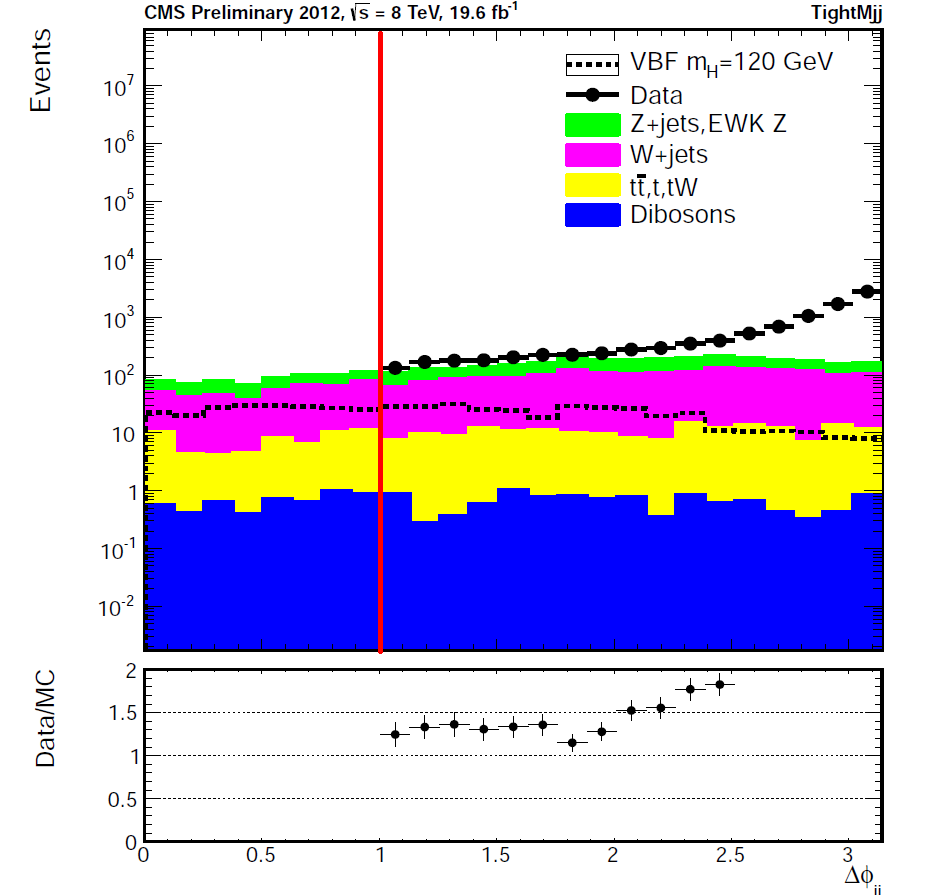
\includegraphics[width=\textwidth]{Images/dphijj_TightMjj_nunu.png}
  \end{subfigure}
  \begin{subfigure}{.5\textwidth}
    \centering
    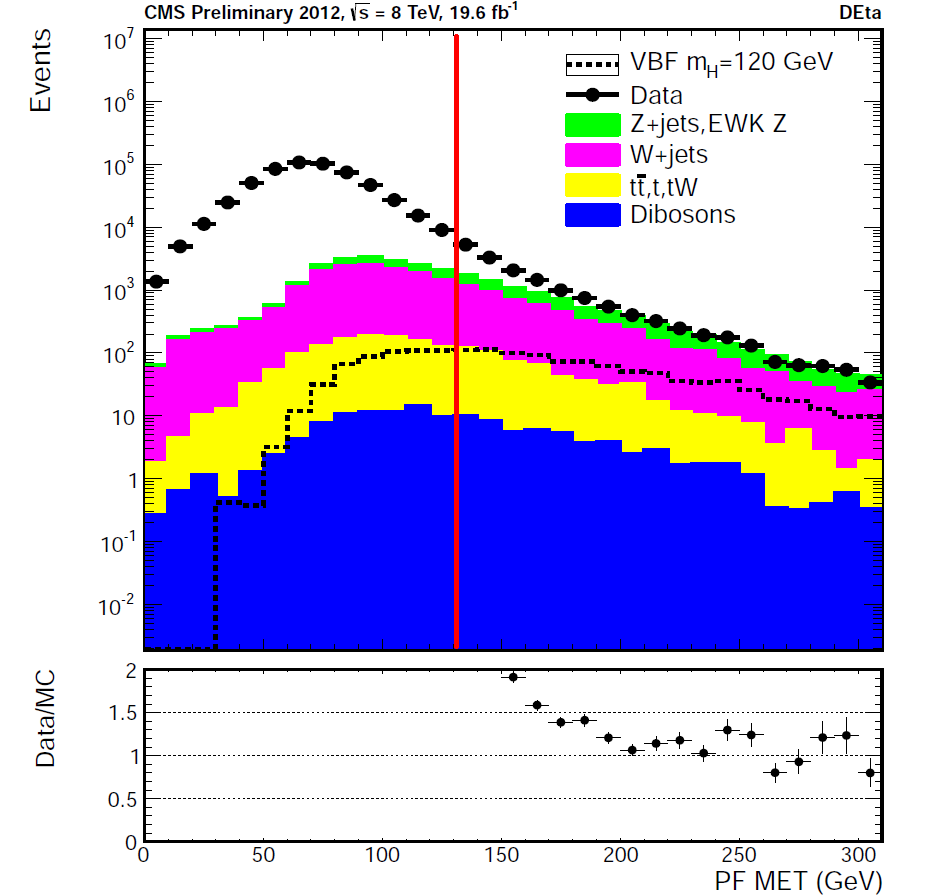
\includegraphics[width=\textwidth]{Images/met_DEta_nunu.png}
  \end{subfigure}
  \caption{Left: plot of azimuthal separation of the two leading jets. Right: plot of missing transverse energy. QCD is not included in these plots due to low MC statistics, and is expected to account for the difference between data and MC prediction. The red line shows the value where a cut is placed in the signal selection. The dashed signal line, shows the expected number of events for a 120 GeV Higgs boson with 100\% invisible branching fraction}
  \label{controlplots}
\end{figure} 

Events that contain electrons (muons) identified by the particle flow algorithm and fulfilling the following criteria are also vetoed, as signal events are not expected to contain leptons:
\begin{equation}
p_{T}>10\,\rm{GeV}, \rm{relative\,\,isolation} < 0.15(0.2), |\eta|<2.4(2.1),
\end{equation}
where relative isolation is defined as the ratio between the objects transverse momentum and the transverse momentum of the other objects within a cone of $\Delta R$ = 0.4, where
\begin{equation}
  \Delta R = \sqrt{(\eta-\eta_{lepton})^{2}+(\phi-\phi_{lepton})^{2}}.
\end{equation}

\subsection{Background estimation}
\label{invbgd}
Even after both sets of cuts have been applied there are still events left from background processes. Due to the hard cuts that have been imposed Monte Carlo samples are not expected to be reliable to provide a good estimation of the number of remaining background events, data driven background estimation techniques must therefore be used for the dominant backgrounds. All of the following data driven techniques use the same basic method:
\begin{itemize}
  \item[1)] A control region which is dominated by the background to be estimated is chosen.
  \item[2)] The assumption is made that, even though the absolute number of events in the Monte Carlo sample is untrustworthy, the ratio of the number of events in the signal region to that in the control region is trustworthy and that the shape of the background distribution is the same in data and MC.
  \item[3)] The number of events in the signal region in data is calculated by multiplying the number of events in the control region by the ratio from step 2.
\end{itemize}

\subsubsection{\boldmath{W+}jets}
The control region used for the $W$ + jets background, where the $W$ boson decays to an electron or muon, is that where the VBF cuts from eqn.~\ref{vbfcuts} are passed and there is exactly one electron (muon) satisfying the following requirements:

\begin{equation}
  \label{vetoleptons}
  p_{T} > 20 \,\rm{GeV}, |\eta|<2.4(2.1),\rm{relative\,\,isolation}<0.1(0.12),
\end{equation}

and the missing transverse energy, which is recalculated after removing the lepton from the event to mimic it having not been detected, is greater than 130 GeV.

The estimated number of events present in the signal region in data is then:
\begin{equation}
  N^{S}_{data} (W\rightarrow e/\mu) = (N^{C}_{data}-N^{C}_{bkg})\frac{N^{S}_{MC}}{N^{C}_{MC}},
\end{equation}
where $N^{S}$ and $N^{C}$ are the number of events in the signal and control regions respectively, and $N^{C}_{bkg}$ is the number of events from minor background sources in the control region which are estimated from top pair, diboson and single-top Monte Carlo samples. 

The current estimate for the number of events in the signal region in data from the $W$ + jets background is $87\pm17$ due to $W$ bosons decaying to electrons, and $105\pm13$ due to $W$ bosons decaying to muons. The errors quoted are statistical errors only, systematic errors are discussed below.

A slightly different method is used for the case where the $W$ decays to a tau. In this case a direct measurement is made in data by using the signal region selection, but additionally requiring a tau lepton, reconstructed using the particle flow approach described in ref.~\cite{tau}, with transverse momentum greater than 20 GeV and pseudorapidity less than 2.3. The number of events selected is then corrected by the efficiency for selecting a tau, taken from MC. This leads to an estimated $135\pm52$ events in the signal region in data, the error quoted is the statistical error combined with the uncertainty on the data to MC scale factor for the tau identification efficiency.

\subsubsection{\boldmath{Z+}jets}
The $Z$ + jets background comes from events where the $Z$ boson decays to two neutrinos. The number of events from this background is estimated using $Z$ + jets events where the $Z$ decays to two muons. The control region criteria are that the VBF cuts from eqn.~\ref{vbfcuts} are passed, there are exactly two muons satisfying the requirements of eqn.~\ref{vetoleptons} and the missing transverse energy, which is recalculated after removing the two muons from the event to mimic them having been neutrinos, is greater than 130 GeV.

The estimated number of events present in the signal region in data is then:
\begin{equation}
  N^{S}_{data} (Z\rightarrow \nu \nu) = (N^{C}_{data}-N^{C}_{bkg})\frac{\sigma(Z\rightarrow\nu\nu)}{\sigma(Z/\gamma^{*}\rightarrow\mu\mu)}\frac{\epsilon^{S}_{VBF}/\epsilon^{C}_{VBF}}{\epsilon_{\mu\mu}}
\end{equation}
where $\epsilon^{S,C}_{VBF}$ is the efficiency of the VBF cuts and $\epsilon_{\mu\mu}$ is the efficiency for selecting two muons. The cross-section ratio is present because dimuon production via an excited photon is indistinguishable from that via a $Z$ boson, so a correction must be made. This method leads to an estimated $162\pm48$ events in the signal region in data, the error quoted is statistical only, but systematic erros from theoretical uncertainties on the cross-section, the jet energy scale and resolution and pileup reweighting are in the process of being calculated.

\subsubsection{QCD multijets}
\label{qcd}
The QCD multijet background analysis presents problems due to the very low number of events in the Monte Carlo samples after the cuts in eqns.~\ref{vbfcuts} and \ref{sigsel}. Because we cannot trust the QCD Monte Carlo we are left with two options; either we must estimate the background from data to a high degree of accuracy, or we must introduce further cuts to make the QCD multijet background small enough that a large relative uncertainty on its estimation is not important. Both options are currently being studied.

In the case of an accurate estimation, the method used is as follows. As shown by Fig.~\ref{qcddiag}, we expect the region where the VBF jets have a high azimuthal separation to be dominated by the QCD multijet background. The control region for the QCD multijet background is therefore defined as those events which pass the cuts in eqn.~\ref{vbfcuts} and also satisfy
\begin{equation}
  \label{qcdcontrol}
  \slashed{E}_{T} > 130 \,\rm{GeV}, \Delta\phi_{jj} >2.6, 
\end{equation}

\begin{figure}[h]
  \centering
  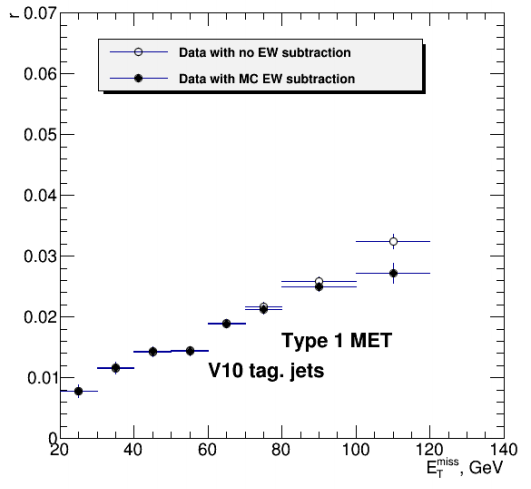
\includegraphics[width=.5\textwidth]{Images/qcdplot.png}
  \caption{QCD extrapolation factor, r, against missing transverse energy cut}
  \label{qcdplot}
\end{figure}

The number of events expected in the signal region is then given by:
\begin{equation}
  N_{S}=(N_{C}-N_{bkg})\cdot r.
\end{equation}
In the above equation r is calculated in the region passing the cuts of eqn~\ref{vbfcuts} and the jet azimuthal separation requirement but not the additional requirements of the QCD control region and is given by:
\begin{equation}
  r = \frac{N_{data} (\Delta\phi_{jj} < 1.0) - N_{bkg} (\Delta\phi_{jj} <1.0)}{N_{data} (\Delta\phi_{jj} >2.6) - N_{bkg} (\Delta\phi_{jj} >2.6)}.
\end{equation}
This method relies on the value of r being constant with increasingly stringent missing transverse energy cuts, initial studies showed that this was the case, however, even after subtraction of other electroweak backgrounds in MC, further investigation, the results of which are shown in Fig.~\ref{qcdplot}, showed an increase in r as the missing transverse energy cut increased. This increase renders this method unusable without further study.

As a result of the issues with estimating the background several techniques are being investigated to implement the other option, reducing the QCD multijet background to a level where a large uncertainty on its estimation is acceptable. Examples of this include a central jet veto, i.e. vetoing events with additional jets between the two VBF jets, as additional jets are not expected in signal events. These studies are ongoing and the method for dealing with the QCD multijet background has not yet been finally determined.

\subsection{Systematic uncertainties}
\label{invsys}
\subsubsection{Jet Energy Scale (JES)}
\label{JES}
The energy of a jet that has been reconstructed by CMS is not necessarily the same as the true energy of the combination of all the particles that make it up. To deal with this, corrections, called the jet energy scale, are applied to jets' four vectors to achieve a uniform response as a function of transverse momentum and pseudorapidity, and to make the ratio of reconstructed jet energy to the true jet energy, on average one. 

The jet corrections can be factorised into several separate corrections. These are: an offset correction, which removes extra energy due to pileup and noise, a MC correction, which corrects for most of the non-uniformity in pseudorapidity and non-linearity and non-compensation in transverse momentum, and residual relative and absolute energy scales, which correct for the remaining non-uniformity and the non-linearity and non-compensation respectively of the detector that is not accounted for by the MC correction \cite{JES/R}.

The offset correction is determined using several different methods, which produce slightly different results. These differences give rise to an uncertainty on the final offset correction that is used. Similarly, the MC correction is sensitive to the MC generator that is used, and also to theoretical considerations such as the parton distribution functions chosen. Again, the differences in final result between these methods give rise to an uncertainty on the JES.

The relative residual correction is calculated using the dijet $p_{T}$ balance technique. This method assumes that the two jets in dijet events have the same transverse momentum, i.e. are balanced, and thus, by selecting events where one of the jets is detected in the barrel and the other in a different pseudorapidity region and comparing their measured transverse momentum, extracts the relative response of the detector as a function of pseudorapidity. There are, however, uncertainties on the response function extracted using this method, primarily due to jet resolution bias. Jet resolution bias occurs because the transverse momentum spectrum of jets falls steeply with increasing transverse momentum, so a barrel jet measured at a particular $p_{T}$ is more likely to have fluctuated up in $p_{T}$ than down, leading to a bias in the result which depends on the jet resolution.

The absolute residual correction is calculated using photon/$Z$+jets events, again assuming that the system is balanced and comparing the value of the reference $Z$ or photon's transverse momentum, which is known to have a peak at a certain mass, to that of the jet system to obtain an absolute calibration. In this case the resolution of the photon/$Z$ boson is good so there is no resolution bias, the method is, however, vulnerable to other uncertainty sources sach as the uncertainty in the photon energy scale \cite{JES/R}.

The combined uncertainty on the JES due to all of the above uncertainties has been calculated and is given as the relative uncertainty on jet transverse momentum as a function of transverse momentum and pseudorapidity. In order to estimate the effect of this combined uncertainty on our background estimations, the analysis of the Monte Carlo samples is rerun with the JES scaled up and down to its $\pm 1 \sigma$ uncertainty limits. Because the momentum of the jets in the event has changed, the missing transverse energy is also expected to change, so this is recalculated after the jets have been scaled. It is also important when carrying out the uncertainty estimation that the two highest transverse momentum jets are selected after the JES has been rescaled, as for some samples up to 3.5\% of events were found to have different leading jets after rescaling.

\begin{figure}[h]
  \begin{subfigure}{.5\textwidth}
    \centering
    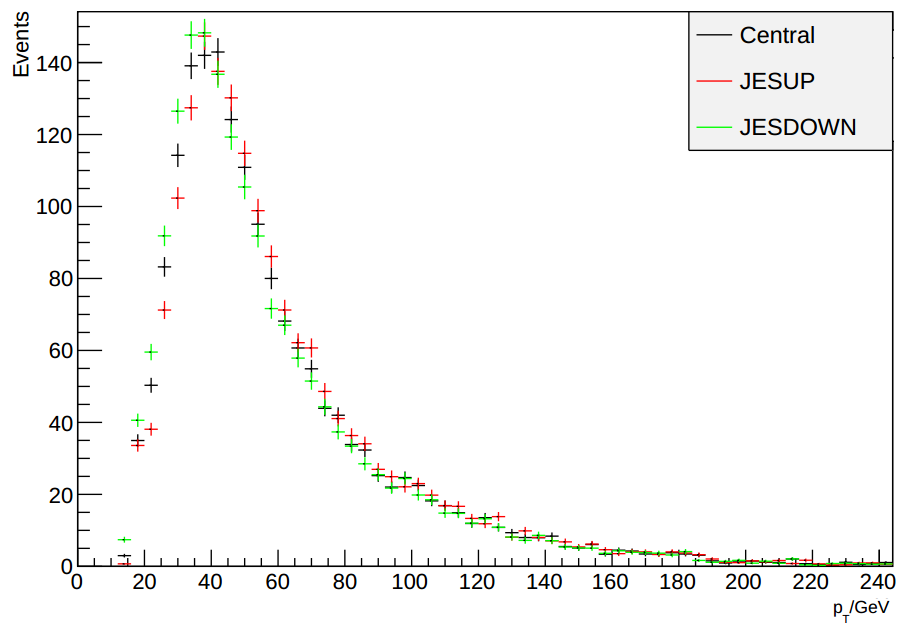
\includegraphics[width=\textwidth]{Images/jescheck.png}
    \caption{}
  \end{subfigure}
  \begin{subfigure}{.5\textwidth}
    \centering
    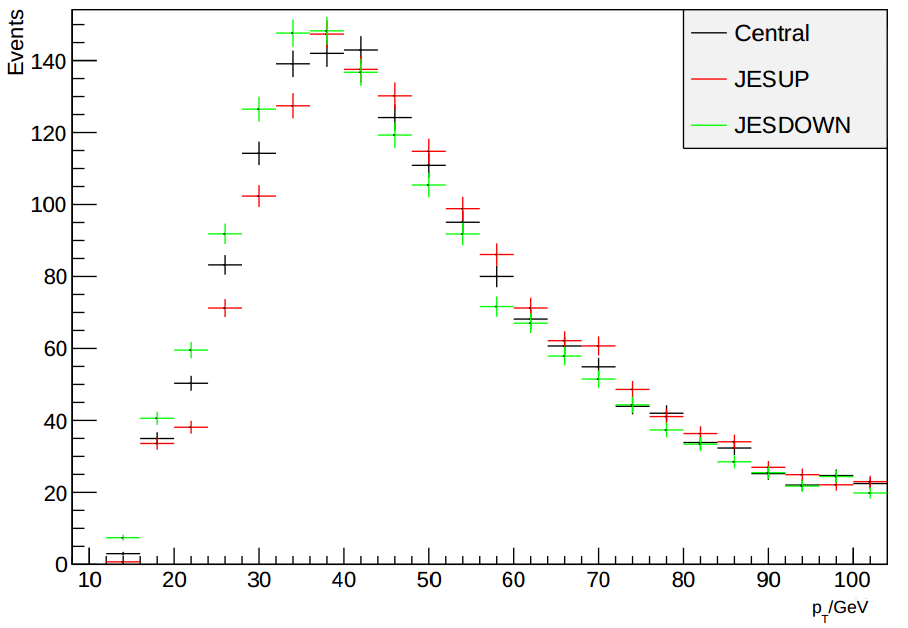
\includegraphics[width=\textwidth]{Images/jescheckzoom.png}
    \caption{}
  \end{subfigure}
  \caption{A plot of the number of events against the second highest $p_{T}$ jet's transverse momentum for nominal JES, JES scaled up (JESUP) and JES scaled down (JESDOWN), for W+Jets Monte Carlo sample}
  \label{jescheck}
\end{figure}

The JES uncertainty is provided as a function of jet transverse momentum and pseudorapidity. Fig.~\ref{jescheck}a shows that this procedure results in a smooth shift in the distribution of jets across the full range of transverse momentum, and thus that the difference in the final number of events selected, shown in Table~\ref{sysnumbers}, after JES rescaling is not just due to a few events with large weights receiving large corrections. Fig.~\ref{jescheck}b shows the same as Fig.~\ref{jescheck}a, but in more detail around the region where the jet transverse momentum cut is placed.

\subsubsection{Jet Energy Resolution (JER)}
\label{JER}
In addition to the average value of the ratio of the reconstructed jet energy to the true jet energy not necessarily being one, the width of the distribution is also not necessarily the same in data and MC, this width is called the jet energy resolution. 

The JER is measured in both data and MC using the dijet balance method, described in Sec.~\ref{JES}, and using a photon + jet balance method. The photon + jet balance method is performed on the sample of events with a single photon and a single jet. The photon is considered to be well measured by the ECAL and, given the transverse momentum of the jet should balance that of the photon, the resolution is then taken to be the width of the distribution of the ratio of the jet's transverse momentum that that of the photon. Both of the methods used have uncertainties, described above for the dijet balance method, and primarily due to limited statistics in the photon + jets sample for the photon + jets method.

Unlike JES, where the corrections from MC to the nominal value in data are provided, for JER there is also the added complication that the correction from the resolution used to produce Monte Carlo samples to the nominal value in data must be done manually. Some change of resolution is therefore necessary to obtain even the nominal Monte Carlo result, these changes in JER are known as smearing. In addition to this central smearing the estimation of an error due to the JER uncertainty is performed, and takes the same form as that for the JES, i.e. the JER is varied to it's better and worse $1 \sigma$ confidence levels and the analysis is rerun.

The prescription used to alter the resolution uses the fact that for Monte Carlo samples the true, `generated', jet energy is known. The difference between the generated and reconstructed transverse momenta is scaled by a correction factor, $c$, according to the following formula:
\begin{equation}
  p_{T new} = max[0,p_{Tgen}+c(p_{T old}-p_{T gen})],
\end{equation} 
where $p_{Tgen}$ is the generated transverse momentum, $p_{Told}$ is the initial reconstructed jet $p_{T}$ and $p_{Tnew}$ is the corrected reconstructed jet $p_{T}$. This method involves no random corrections, so it produces the same jets every time it is applied, making cross-checks easier to perform.

However, not all jets are well matched to a generator level jet. For these jets a random correction is necessary. The technique used is to add a random gaussian fluctuation to the jets transverse energy with width $\sqrt{(c^{2}-1)}\sigma_{MC}$, where c is the same correction factor used for the deterministic method above. 

Other than being random, and thus making jets harder to compare for cross-checking purposes, this method also has the disadvantage that it can only be used to worsen the resolution. For the nominal resolution and the estimate of the effect of worse resolution than the nominal value this is not a problem, as the Monte Carlo resolution must be worsened to match the data anyway. Unfortunately, for the estimate of the effect of better than nominal resolution the MC resolution must be slightly improved for jets in some pseudorapidity regions. However, the difference between the better resolution and the unsmeared MC resolution is very small, so in this case the unsmeared MC can be used.

For the numbers presented in Table~\ref{sysnumbers} only the deterministic generator level jet matching technique has been used. It is intended that in the future the random gaussian smearing method will be implemented as well. 

\subsubsection{Other uncertainties}
Other uncertainties expected to have an effect on the background estimation for the Higgs to invisible analysis are the pileup weight, unclustered energy uncertainties. The effect of these uncertainties on the Higgs to invisible analysis is still to be investigated, but is expected to be small. The estimation of the first two of these uncertainties will be carried out in the same way as the estimation of the uncertainty on the JES, the quantities will be varied to their upper and lower one sigma confidence limits and the analysis will be rerun. The origin of these two uncertainties will now be discussed.

As mentioned above, pileup is particles from interactions other than the interaction of interest. The distribution of the number of interactions from pileup in each event that is generated in MC is not the same as that measured in data, so the pileup weight is applied to correct this difference, with MC events with numbers of pileup interactions that are more common in MC than data having low weights and vice versa. However, there are uncertainties on the measurement of the number of pileup events in data, from the uncertainties on the total luminosity and inclusive cross-section measurements, and thus the weights have an associated uncertainty \cite{incxsec,lumimeas}.

Energy deposits in the calorimeters which are not identified by the particle flow reconstruction as being part of an object, such as a jet or lepton, still have an impact on the missing transverse energy calculation. Furthermore, in exactly the same way as for jets, the unclustered energy measured by the detector is not necessarily that which is truly deposited. A scale factor is therefore used, like the JES factor for jets, to corrected the measured distribution. Again, as for the JES the measurement of this scale factor has an associated uncertainty, in this case from the resolution of the calorimetry systems. 

\subsubsection{Results of Sytematic Uncertainty Estimations}
\begin{table}[h]
  \centering
  \begin{tabular}{|l|| c| c| }
    \hline
    $N_{W\rightarrow e\nu}^{data}$ & Electron & Muon \\
    \hline
    Central num. of events & 87 & 105  \\
    \hline
    Statistical & $\pm$20\% & $\pm$12\% \\
    JES scaled up & -4\% & +5\% \\
    JES scaled down & +4\% & +2\% \% \\
    JER made better & +3\% & -1\%  \\
    JER made worse & +7\% & +7\%  \\
    \hline
  \end{tabular}
  \caption{The contributions of the currently estimated uncertainties on the $W$ + jets background estimation}
  \label{sysnumbers}
\end{table}
As can be seen from Table~\ref{sysnumbers} whilst the errors due to the currently estimated systematic uncertainties are not insignificant, especially in the case of $W$ bosons decaying to electrons, the overall uncertainty is still dominated by the statistical error.



\section{Combination of Higgs boson decay channels}
\label{combs}
In order to establish whether what has been found at CMS is a SM Higgs boson it is important to combine the results of the different searches and compare them with the SM predictions. In order to do this the errors, both statistical and systematic, on the various analyses and their correlations must be taken into account as well as each channel's results.

\subsection{Methods}
The CMS combinations group compares the data to standard model predictions in three main ways: limits are placed on regions where we can exclude a standard model Higgs boson, excesses over background are characterised and signal model parameters are extracted and compared to their standard model values \cite{hcpcomb2012}. A general methodology for doing this has been developed by ATLAS and CMS which is described in refs.~\cite{comb2011,lhccomb1} and described below are the methods used for performing the above three data to signal comparisons as they appear in ref.~\cite{hcpcomb2012}.


\subsubsection{Exclusion limits}
For setting exclusion limits the CL$_{s}$ statistic is used, which is a function of the profile likelihood ratio, q$_{\mu}$, defined as:
\begin{equation}
  q_{\mu} = -2 \ln\frac{\mathcal{L}(obs|\mu \cdot s + b,\hat{\theta}_{\mu})}{\mathcal{L}(obs|\hat{\mu} \cdot s + b,\hat{\theta})}\,,
\end{equation}
where $\mathcal{L}$ is the likelihood, $obs$ is the observation, s is the SM expected Higgs signal and b is the background. $\mu$ is a signal strength modifier which is 1 for a SM Higgs boson and 0 for the background only case. $\theta$ are nuisance parameters, such as systematic uncertainties, which include the errors and any correlations between them. $\hat{\mu}$ and $\hat{\theta}$ are the values of $\theta$ and $\mu$ where the likelihood, $\mathcal{L}$, is maximised, and $\hat{\theta}_{\mu}$ is the $\theta$ that maximises the likelihood for a given $\mu$. The profile likelihood ratio therefore describes how likely a given signal strength is compared to the most likely signal strength.

The definition of CL$_{s}$ is
\begin{equation}
  CL_{s} = \frac{P(q_{\mu}\geqslant q_{\mu}^{obs} | \mu \cdot s + b)}{P(q_{\mu}\geqslant q_{\mu}^{obs}|b)}\,,
\end{equation}
Where the method of determining the probability, $P$, varies. The region in which a signal strength $\mu \cdot s$ is excluded with $1 - \alpha$ confidence is then the region for which CL$_{s}$ is less than or equal to $\alpha$, i.e. when the background hypothesis is $1/\alpha$ times more likely than the signal hypothesis we exclude the signal hypothesis with $1 - \alpha$ confidence.

\subsubsection{Characterising excesses}
When the signal model cannot be excluded, the observed excess of events over that expected from background is characterised by calculating q$_{0}$ by setting $\mu$ to zero in q$_{\mu}$. Next, p$_0$, which is defined as
\begin{equation}
p_{0} = P(q_{0} \leqslant q_{0}^{obs}|b)\,,
\end{equation}
is calculated and then the statistical significance of the excess, Z in units of standard deviations, is defined as the value of Z for which:
\begin{equation}
  p_{0}=\int_{Z}^{+\infty}\frac{1}{\sqrt{2\pi}}\exp(-x^{2}/2)dx\,.
\end{equation}

\subsubsection{Signal parameter determination}
In order to extract confidence limits on signal model parameters the profile likelihood ratio is used again, in this case it is defined as:
\begin{equation}
  q(a) = -2\ln\frac{\mathcal{L}(obs|s(a)+b,\hat{\theta}_{a})}{\mathcal{L}(obs|s(\hat{a})+b,\hat{\theta})}\,,
\end{equation}
where a is the parameter of interest, s, b and $\theta$ are defined as above, $\hat{a}$ and $\hat{\theta}$ are the values of $\theta$ and a at the global maximum of $\mathcal{L}$ and $\hat{\theta}_{a}$ is the $\theta$ that maximises $\mathcal{L}$ for the given a.

The one sigma and two sigma confidence limits on the parameter are then the values of a for which q(a) is equal to 1.00 or 3.84 respectively treating all other unconstrained parameters as nuisance parameters. It is also possible to produce confidence limit contours for two parameters by taking q($a_{i}$,$a_{j}$), however the values of q corresponding to one sigma and two sigma contours are now 2.30 and 6.00 respectively.

\subsection{Uncertainty pruning}
\label{uncprune}
All of the above techniques rely on evaluating the minima of the likelihood and comparing this value to its value for other values of the parameters. Minimizing and profiling likelihood functions is therefore a very important part of the combinations analysis. It is also a very computing intensive process; so simplifying the likelihood function, or its parameter set, can assist greatly in carrying out the analysis, as fewer minimizations will fail to converge or be aborted due to overruning the time limits on computing resources.

One method for simplifying the likelihood is to identify nuisances whose inclusion has only a small effect on the final value of the test statistic and remove them from the set of parameters that is profiled. This process is called `pruning'.

There are several methods of estimating the effect of a particular nuisance on the final result. One way of doing this is to refit neglecting one nuisance at a time. Unfortunately, given that each fit takes a considerable amount of time and for some of the decay modes there are several hundred nuisances, the time taken to do this is prohibitively large.

Another method is to prune nuisances based on a quantity called the pull. The pull is defined as follows:
\begin{equation}
  \rm{pull}\,=\frac{x_{fit}-x_{measured}}{\sigma_{fit}},
\end{equation}
i.e. the significance of the difference between the best fit value of the nuisance and its measured value \cite{cdfpulls}.

However, pruning nuisances only by pull has the problem that large uncertainties with a small pull can still have a large effect on the final result. Deciding which uncertainties to prune using the pull multiplied by the size of the uncertainty due to the nuisance accounts for this issue whilst still only requiring one fit. Due to these advantages this is the method that has been used for the following results.

In the study shown below each decay mode was pruned separately, this introduces an additional issue because some nuisances are correlated between decay modes and, whilst they may only have a small effect in one channel, they must still be included, due to their effect in another. Therefore, all nuisances appearing in multiple decay modes were not pruned regardless of whether they had a large or small effect on a particular decay mode.

\begin{figure}
  \begin{subfigure}{.5\textwidth}
    \centering
    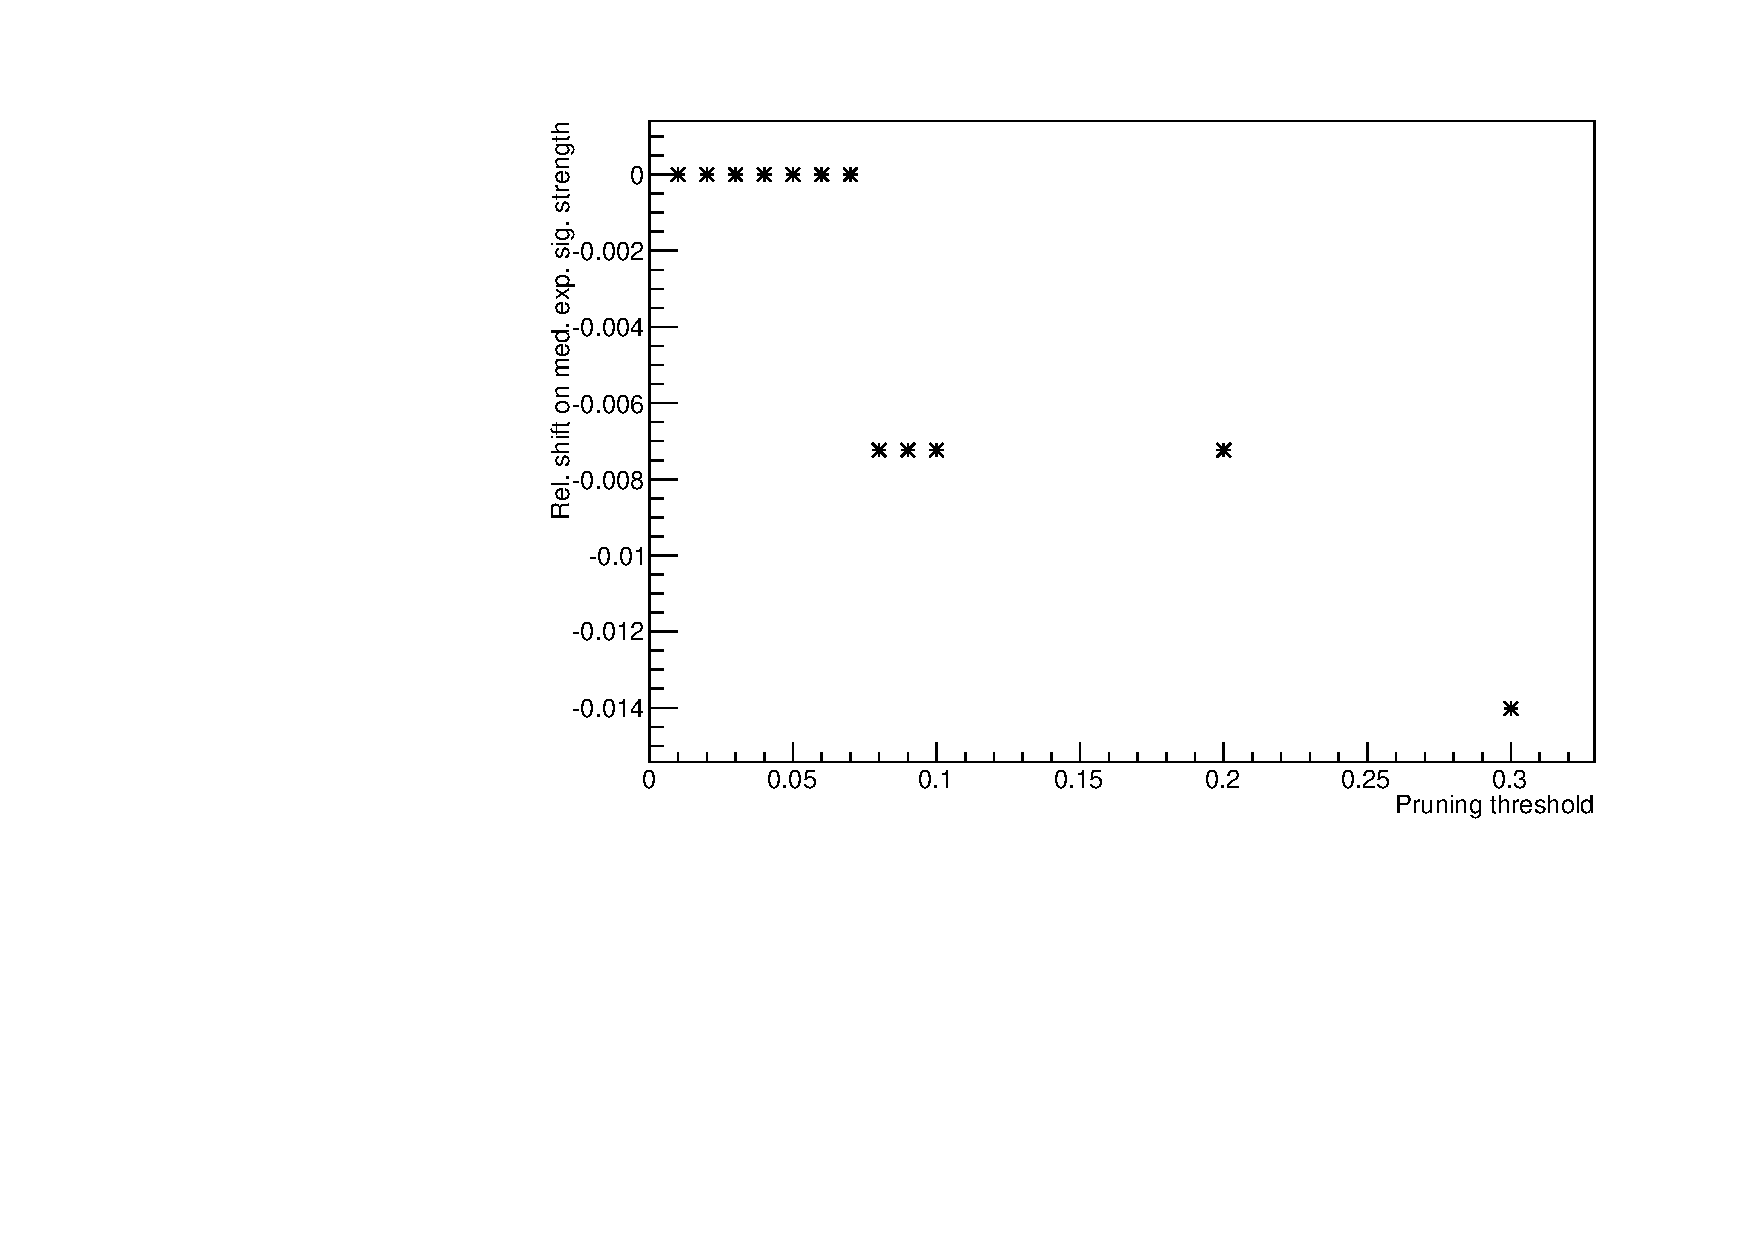
\includegraphics[width=\textwidth]{Images/hwwshift.pdf}
    \caption{}
  \end{subfigure}
  \begin{subfigure}{.5\textwidth}
    \centering
    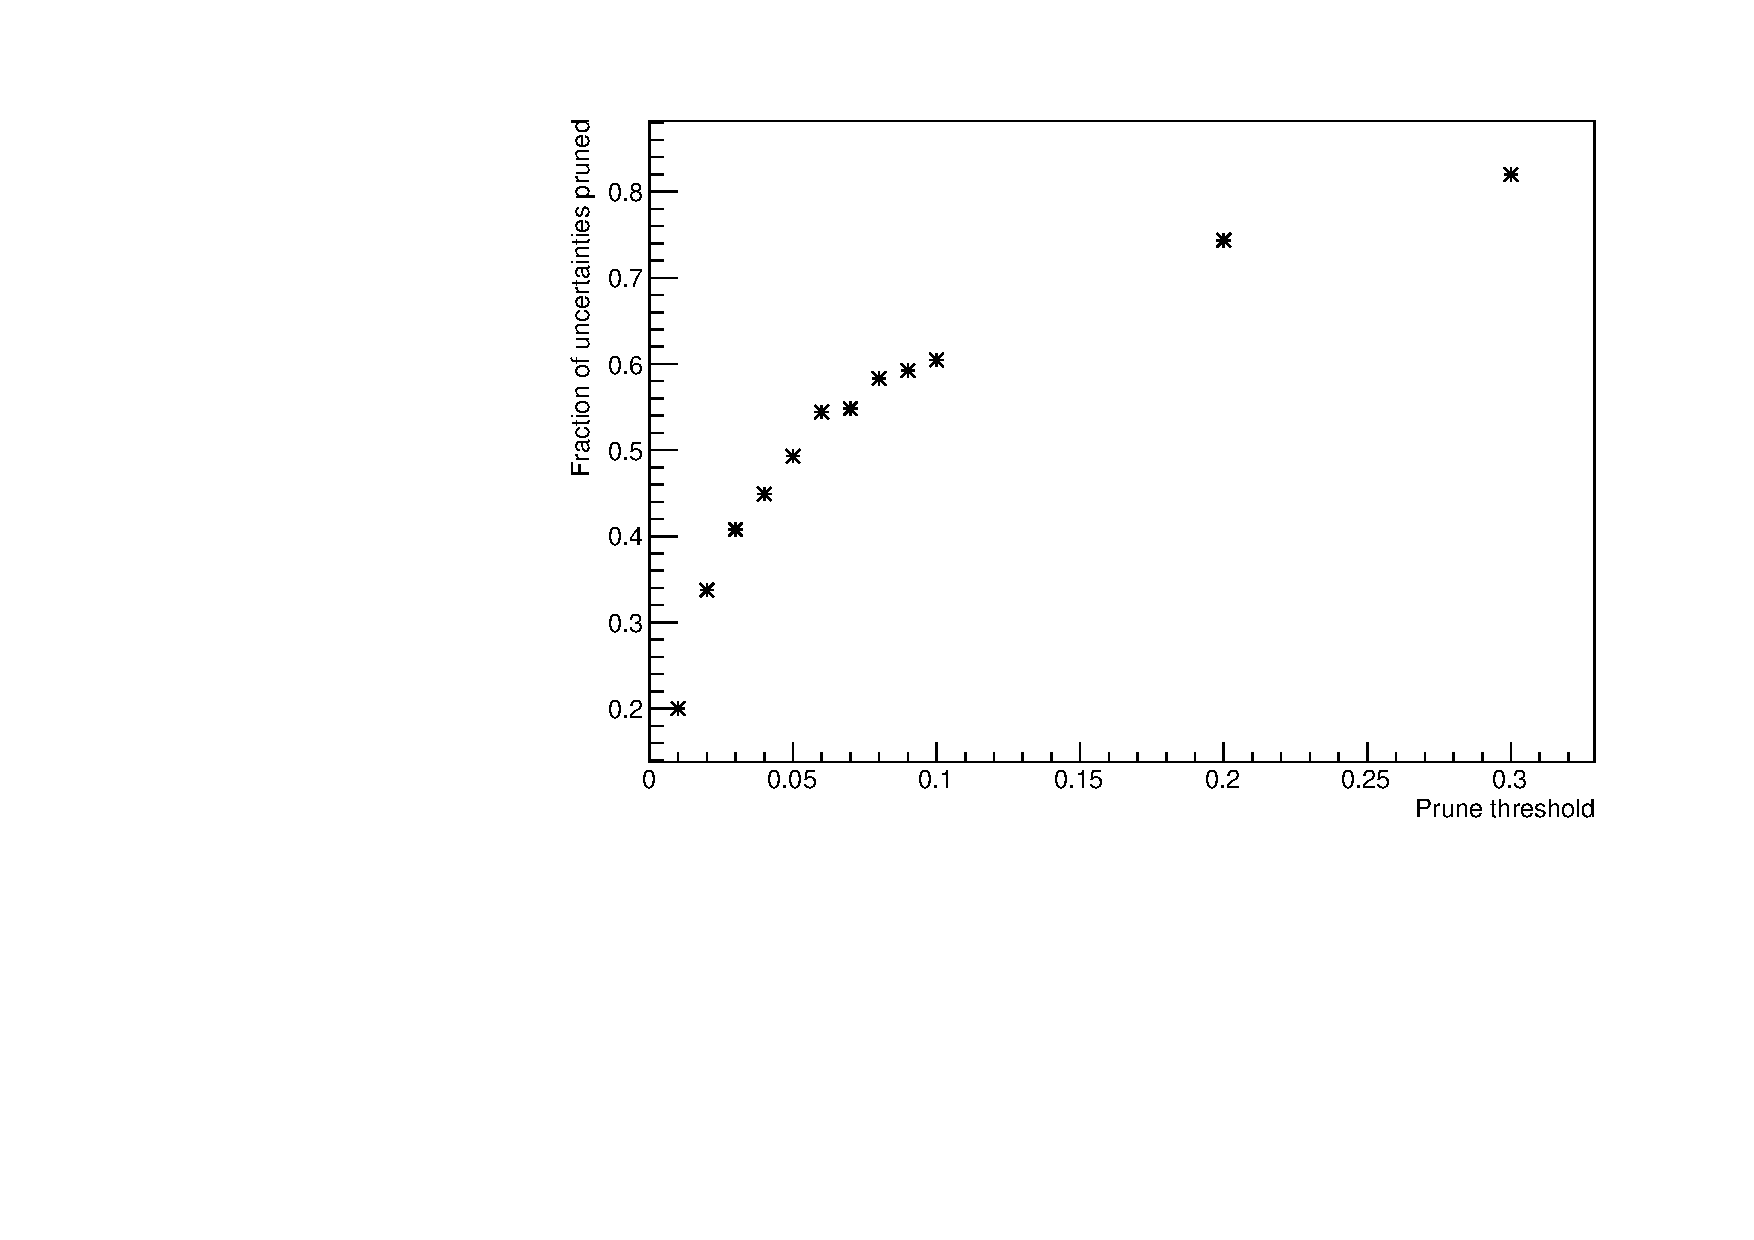
\includegraphics[width=\textwidth]{Images/hwwprop.pdf}
    \caption{}
  \end{subfigure}
  \caption{Plots showing the impact of uncertainty pruning in the Higgs to $WW$ channel at a mass of 140 GeV. a) The change in the median expected signal strength divided by the result obtained without pruning plotted against the pruning threshold. b) The fraction of the uncertainties that are pruned plotted against the pruning threshold }
  \label{pruneplots}
\end{figure}
The pull of each nuisance was evaluated and multiplied by the uncertainty due to the nuisances, and a list was made of nuisances where this value was below a given threshold. The best fit value of the relative median signal strength was then recalculated after pruning the uncertainties. This procedure was repeated at several pruning thresholds. Fig.~\ref{pruneplots} shows that even when quite a large proportion of the uncertainties are not included in the fit, the shift on the result can still be at around the one percent level. Furthermore, for the channel shown in Fig.~\ref{pruneplots}, Higgs to $WW$, the time taken to carry out the fit for the signal strength for a pruning threshold of 0.3 took only 23 seconds, half the time of the unpruned fit.

The results do vary from channel to channel, for instance in the Higgs to $b\bar{b}$ channel the relative shift in the median expected signal strength is 6\% for even a pruning threshold of 0.01. However, for Higgs to $\gamma\gamma$ at a pruning threshold of 0.3 no shift is seen, and the fitting time is again reduced by a factor of approximately two from 31 minutes for the unpruned fit to 17 minutes with pruning.

\section{Conclusions}
The Higgs to invisible analysis of prompt data from CMS has been presented, and the outstanding issues have been outlined, namely that there are still some systematic uncertainties to be estimated (see Sec.~\ref{invsys}), and that the method for the QCD multijet background estimation has not been finalised (see Sec.~\ref{qcd}). The author, assisted in the estimation of the $W$ + jets background, and performed the estimations of the systematic uncertainties presented in Sec.~\ref{invsys}

Once the analysis of the prompt data has been completed it is planned that the analysis will be performed again using the parked data discussed in Sec.~\ref{trigcomp}. The triggers present in the parked data are less stringent, at HLT level the missing transverse energy threshold is lowered to 35 GeV, the jet $p_{T}$ threshold is lowered to 35 GeV and the $M_{jj}$ threshold is lowered to 700 GeV, which should result in fewer signal events being lost and larger numbers of events in the control regions used for background estimation, and thus reduce statistical errors \cite{jimtalk}. It is also planned to change from a counting experiment to a shape based analysis, taking into account the distribution of events in the signal region rather than just the number of them that remain after all cuts.

The process of producing a combined result for all Higgs boson decay modes has also been presented, and it has been demonstrated that, in some channels, pruning of nuisances can significantly reduce the time taken to minimise and profile likelihood functions, whilst not affecting the results by a large amount (see Sec.~\ref{uncprune}). Once the studies of this method are completed, and pruning thresholds have been finalised, it is envisaged that this pruning will be used to assist in placing exclusion limits on second Higgs bosons. Pruning is expected to be particularly helpful for this process because carrying out fits at masses other than that of the Higgs boson that has already been discovered is a process where currently many minimisations fail due to the complexity of the likelihood function.




\begin{thebibliography}{999}
\bibitem{glashow}S. Glashow, ``Partial-symmetries of weak interactions'', Nucl. Phys. 22 (1961) 579.
\bibitem{weinberg}S. Weinberg, ``A Model of Leptons'', Phys. Rev. lett. 19 (1967) 1264.
\bibitem{salam}A. Salam, ``Weak and electromagnetic interactions,'', in: N. Svartholm (Ed.), Elementary Particle Physics: Relativistic Groups and Analyticity, Prodeedings of the Eighth Nobel Symposium, Almquvist and Wiskell, 1968, p. 367.
\bibitem{wdiscovery} UA1 Collaboration, ``Experimental observation of isolated large transverse energy electrons with associated missing energy at $\sqrt{s} = 540\,\rm{GeV}$,'' Phys. Lett. B122 (1983) 103. 
\bibitem{zdiscovery} UA1 Collaboration,  ``Experimental Observation of Lepton Pairs of Invariant Mass Around 95 GeV at the CERN SPS Collider'', Phys. Lett. B126 (1983) 398. 
\bibitem{englertbrout} F. Englert, R. Brout, ``Broken Symmetry and the Mass of Gauge Vector Mesons'', Phys. Rev. Lett. 13 (1964) 321.
\bibitem{higgs1} P.W. Higgs, ``Broken symmetries, massless particles and gauge fields'', Phys. Lett. 12 (1964) 132.
\bibitem{higgs2} P.W. Higgs, ``Broken Symmetries and the Masses of Gauge Bosons'', Phys. Rev. lett. 13 (1964) 508.
\bibitem{guralniketc} G. Guralnik, C. Hagen, T.W.B. Kibble, ``Global Conservation Laws and Massless Particles'', Phys. Rev. Lett. 13 (1964) 585.
\bibitem{higgs3} P.W. Higgs, ``Spontaneous Symmetry Breakdown without Massless Bosons'', Phys. Rev. 145 (1966) 1156.
\bibitem{kibble} T.W.B. Kibble, ``Symmetry breaking in non-Abelian gauge theories'', Phys. Rev. 155 (1967) 1554.
\bibitem{atlasdiscovery} ATLAS Collaboration, ``Observation of a new particle in the search for the Standard Model Higgs boson with the ATLAS detector at the LHC'', Phys. Lett. B716 (2012) 1.
\bibitem{cmsdiscovery} CMS Collaboration, ``Observation of a new boson at a mass of 125 GeV with the CMS experiment at the LHC'', Phys. Lett. B 716 (2012) 30.
\bibitem{lhc} L. Evans, P. Bryant (Eds.), ``LHC Machine'', JINST. 3 (2008) S08001.
\bibitem{lhchxswg} LHC Higgs Cross Section Working Group, S.~Dittmaier, C.~Mariotti, G.~Passarino, and R.~Tanaka (Eds.), 
  {\sl Handbook of LHC Higgs Cross Sections: 2. Differential Distributions}, 
  CERN-2012-002 (CERN, Geneva, 2012), {\tt arXiv:1201.3084 [hep-ph]}.
\bibitem{zeppenfeld} D. Zeppenfeld, ``Observing an invisible Higgs boson'', Phys. Lett. B 495 (2000) 147.
\bibitem{susy} G. Belanger et al, ``The MSSM Invisible Higgs in the light of dark matter and g-2'', Phys. Lett. B 519 (2001) 93.
\bibitem{higgworkgroup2001} Girolamo et al, ``The Higgs Working Group: Summary report, C. Experimental Observation of an invisible Higgs Boson at LHC'', arXiv:hep-ph/0203056 (2001).
\bibitem{extradim} N. Arkani-Hamed et al, ``The Hierarchy problem and new dimensions at a millimeter'', Phys. Lett. B 429 (1998) 263.
\bibitem{atlastdr} ATLAS Collaboration, ``The ATLAS experiment at the CERN Large Hadron Collider'', JINST. 3 (2008) S08003.
\bibitem{cmstdr} CMS Collaboration, ``The CMS experiment at the CERN LHC'', JINST. 3 (2008) S08004.
\bibitem{hcal} CMS Collaboration, ``Energy Response and Longitudinal Shower Profiles Measured in CMS HCAL and Comparison with GEANT4'', CMS NOTE 2006/143.
\bibitem{parkeddata} Z. Demiragli, CMS triggers for some ``Unexpected Higgs Decays'', Higgs-Exo Workshop 04/02/2013.
\bibitem{wlcg} Ian Bird, ``Computing for the Large Hadron Collider'', Annual Review of Nuclear and Particle Science 61 (2011) 99.
\bibitem{particleflow} CMS Collaboration, ``Particle-Flow Event Reconstruction in CMS and Performance for Jets, Taus, and $E_{T}^{miss}$'', CMS Physics Analysis Summary PFT-09-001 (2009)
\bibitem{comb2011} CMS Collaboration, ``Combined results of searches for the standard model Higgs boson in pp collisions at $\sqrt{s} = 7 \,\rm{TeV}$'', Phys. Lett. B 710 (2012) 26.
\bibitem{moriondcomb} CMS Collaboration, ``Measurements of the properties of the new boson with a mass near 125 GeV'', CMS Physics Analysis Summary HIG-13-005 (2013)
\bibitem{susyprimer} S. Martin, ``A Supersymmetry Primer'', arXiv:hep-ph/9709356.

\bibitem{bds} Y. Bai et al, ``Measuring the Invisible Higgs Width at the 7 and 8 TeV LHC'', arXiv:1112.4496.
\bibitem{jimtalk} J. Brooke, ``CMS VBF H$\rightarrow$ Invisible'', Higgs-Exo Workshop 04/02/2013.
\bibitem{tau} CMS Collaboration, ``Performance of tau reconstruction algorithms in 2010 data collected with CMS'', CMS Physics Analysis Summary TAU-11-001 (2011)
\bibitem{JES/R} CMS Collaboration, ``Determination of Jet Energy Calibration and Transverse Momentum Resolution in CMS'', JINST. 6 (2011) P11002
\bibitem{incxsec} CMS Collaboration ``Measurement of the inclusive production cross sections for forward jets and for dijet events with one forward and one central jet in pp collisions at $\sqrt{s}=7$ TeV'', JHEP. 06 (2012) 36.
\bibitem{lumimeas} CMS Collaboration ``Absolute Calibration of the Luminosity Measurement at CMS: Winter 2012 Update'', CMS Physics Analysis Summary SMP-12-008 (2012)
\bibitem{cdfpulls} L. Demortier and L. lyons, ``Everything you always wanted to know about pulls'', CDF/ANAL/PUBLIC/5776 (2002) 
\bibitem{hcpcomb2012} CMS Collaboration, ``Combination of standard model Higgs boson searches and measurements of the properties of a new boson with a mass near 125 GeV'', CMS PAS HIG-12-045 (2012).
\bibitem{lhccomb1} ATLAS and CMS Collaborations, LHC Higgs Combination Group, CMS NOTE 2011/005.


\end{thebibliography}

\end{fmffile}
\end{document}
